\pdfoutput=1

\documentclass{l4proj}

%
% put any packages here
%
\usepackage{mathtools}
\usepackage{amsmath}
\usepackage{amsthm}

%definitions and theorems
\theoremstyle{definition}
\newtheorem{myDef}{Definition}
%

\begin{document}
\title{Implementation of Novel Subgraph Query Processing methods within GraphX}
\author{Iva Stefanova Babukova}
\date{March 20, 2016}
\maketitle

\begin{abstract}
The GraphX system has recently been developed at Berkeley, over the Spark massively-parallel data processing system, as a system for high performance analytics over graph data. It is currently an important tool for graph-analytic tasks, which are core to many data science endeavours. 
At the same time, graph datasets have become increasingly popular, used to model applications from numerous domains from social networks to biology and bioinformatics. 
The goal of this project is to design, implement, and test an algorithm for subgraph queries, on top of GraphX.
\end{abstract}

\educationalconsent
%
%NOTE: if you include the educationalconsent (above) and your project is graded an A then
%      it may be entered in the CS Hall of Fame
%
\tableofcontents
%==============================================================================

\chapter{Introduction}
\pagenumbering{arabic}
The first page, abstract and table of contents are numbered using Roman numerals. From now on pages are numbered
using Arabic numerals. Therefore, immediately after the first call to $\backslash$chapter we need the call
$\backslash$pagenumbering$\{$arabic$\}$ and this should be called once only in the document. 

The first Chapter should then be on page 1. You are allowed 50 pages for a 30 credit project and 35 pages for a 
20 credit report. This includes everything up to but excluding the appendices and bibliograph, i.e. this is a limit on
the body of the report.

You are not allowed to alter text size (it is currently 11pt) neither are you allowed to alter the margins.

Note that in this example, and some of the others, you need to execute the following commands the first time you process the files.
Multiple calls to pdflatex are required to resolve references to labels and citations. The file bib.bib is the bibliography file.

\begin{verbatim}

            > pdflatex example0
            > bibtex example0
            > pdflatex example0
            > pdflatex example0

\end{verbatim}


\section{First Section in Chapter}
Owner/Supervisor: Peter Triantafillou
*Suitable as a Software Engineering project.

Description: 
The GraphX system has recently been developed at Berkeley, over the Spark massively-parallel data processing system, as a system for high performance analytics over graph data. It is currently an important tool for graph-analytic tasks, which are core to many data science endeavours. 

At the same time, graph datasets have become increasingly popular, used to model applications from numerous domains from social networks to biology and bioinformatics. 

This is a project best suited for one or a team of two L4 students. 
The goal of this project is to design, implement, and test a (set of) algorithms for subgraph queries, on top of GraphX. As subgraph querying currently escapes GraphX, we hope with this project to contribute, test, and evaluate such a solution, based on recent research results achieved by our group's PhD students. 

The L4 students will be closely collaborating with PhD students to implement subgraph processing methods into GraphX. 

[1] https://amplab.cs.berkeley.edu/tag/spark/ 
(see the GraphX related papers in this site).

Special Requirements : 
Strong coding skills are required.

\chapter{The Fox and Dog}
The quick brown fox jumped over the lazy dog.
The quick brown fox jumped over the lazy dog.


\section{The Fox Jumps Over}
The quick brown fox jumped over the lazy dog.
The quick brown fox jumped over Uroborus (Figure \ref{uroborus}).


%\vspace{-7mm}
\begin{figure}
\centering
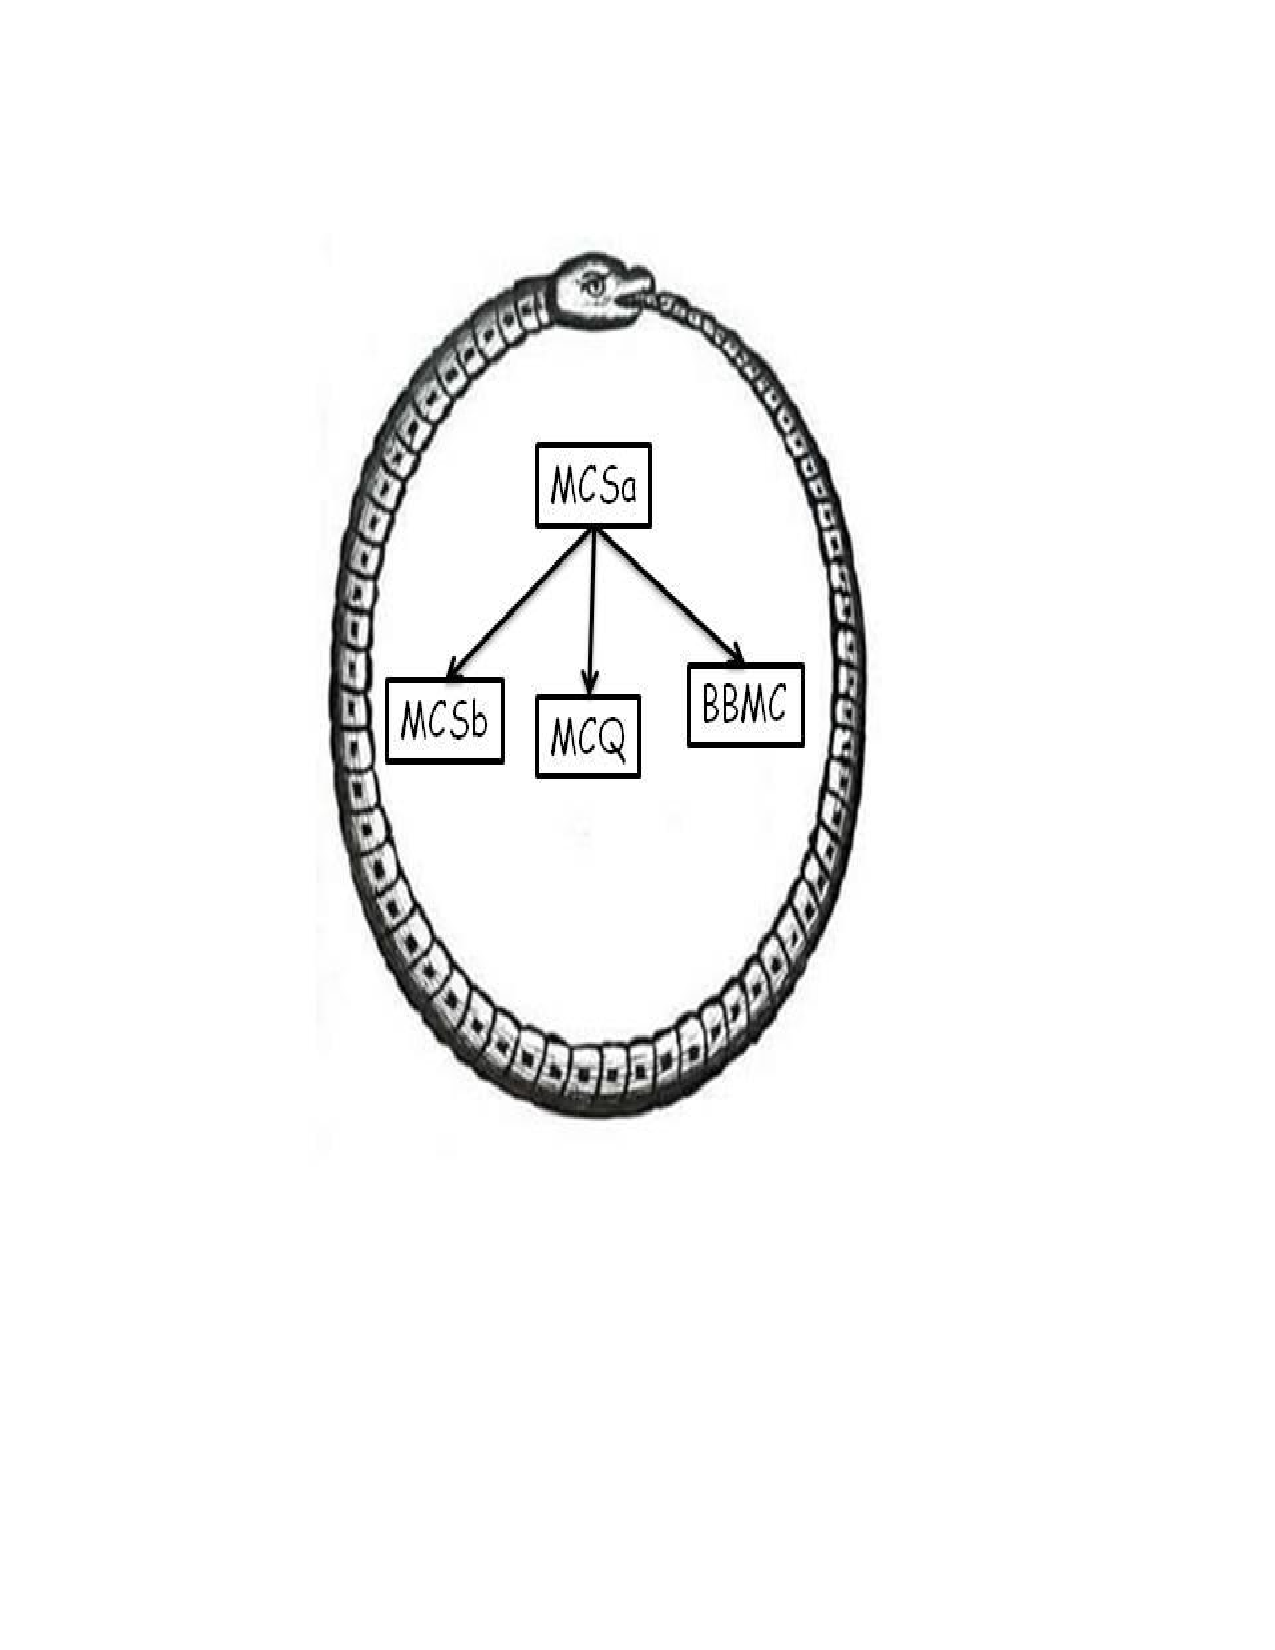
\includegraphics[height=9.2cm,width=13.2cm]{uroboros.pdf}
\vspace{-30mm}
\caption{An alternative hierarchy of the algorithms.}
\label{uroborus}
\end{figure}

The quick brown fox jumped over the \cite{ctindex} lazy dog. \cite{rdds}
The quick brown fox jumped over the lazy dog. \cite{freqStructBasedIndexing}
The quick brown fox jumped over \cite{ckt} the lazy dog.
The quick brown fox jumped over \cite{graphX} the lazy dog.


\section{Assessment criteria}
Has the student surveyed relevant
research literature? Has he/she
analysed the research problem, and
devised a suitable approach for solving
it? 

Has the research been conducted well? Does it show evidence of original thinking? Are there significant errors? Might the research be worth of publication, perhaps after revision?

Has the student critically evaluated and analysed the research results? Does
he/she understand their significance? Does he/she have good suggestions for
further work? 

Is the dissertation complete, well organised, and literate? Does it clearly
explain the problem, and how the software was designed, implemented, tested, and evaluated? Does it contain a bibliography and proper citations? 

Did the student complete a one-page summary of the project satisfactorily?
Did the student attend meetings, and engage effectively with the supervisor?

Did the content reflect a knowledge and understanding of the work done? Were questions handled well? Were visual aids used effectively? Was the delivery fluent and confident, with good eye contact?

\chapter{Introduction}
    \section{Aims and motivation}
        \begin{itemize}
            \item graphs are widely used nowadays to represent data
            \item the graph containment problem is widely addressed in many areas of science: genetics, chemistry, XML documents, images, fraud detection and prevention (there was an article in nature about this)
            \item graph indexing can help us reduce the waiting time
            \item we have a lot of data that often can't be processed in memory by one machine
            \item spark is an engine that allows us to perform cluster computing and load data in-memory and share it across many clusters
            \item graphx is like spark, but has special optimizations for graphs
            \item make graph indexing in java, no concurrency and see the trade off between various indexing approaches
            \item make graph indexing in spark, vary the number of worker threads, measure performance and decide what is best
        \end{itemize}
        
        In the core of many graph-related applications, lies a common and critical problem: \textit{how to efficiently process graph queries and retrieve related graphs}. In some cases, the success of an application directly relies on the efficiency of the query processing system.  
        
        Applications:
        \begin{itemize}
        \item genome sequencing: find mutations responsible for rare diseases -- nature vol 527 no 7576
        \item treating diseases like cancer: screen a patient's tumor for a set of biomarkers to choose the best treatment to fight the particular cancer -- nature vol 527 no 7578
        \end{itemize}
    \section{Background}
        \subsection{Methodologies}
    \section{Preliminaries}
        In this section, we introduce preliminary concepts and outline the main concepts and problems addressed in the document. In definition \ref{def:graphFormat} we explain the format of all graphs used in the document.

        \begin{myDef}[Graph Format]
        \label{def:graphFormat}
        A graph G = (V, E, L, $\lambda$) is defined as an undirected labeled graph where V is the set of vertices, E is the set of edges(unordered pair of vertices), L is the set of labels, and $\lambda$ is a labeling function, $\lambda$ : V $\cup$ E $\rightarrow$ L, that assigns labels to vertices and edges.
        \end{myDef}
        
        \begin{myDef}[Graph Isomorphism]
        
        \end{myDef}

        \begin{myDef}[Subgraph Isomorphism]
        \label{def:subgraphIsomorphism}
        Given a graph database T of target graphs $t^{}_0$, $t^{}_1$, $t^{}_2$ \ldots $t^{}_i$, where \textit{i} is the number of target graphs in T, and a pattern graph P, find all targets in T that have P as a subgraph.
        \end{myDef}
        
        \begin{myDef}[Subgraph]
        \label{def:subgraph}
        A graph whose vertices and edges are a subset of another graph.
        \end{myDef}
        
        \begin{myDef}[Graph Query Processing]
        \label{def:graphQueryProcessing}
        Given a graph database D = $\{$ $g^{}_0$, $g^{}_1$, $g^{}_2$ \ldots $g^{}_n$ $\}$ and a pattern graph p, it returns the query answer set $D^{}_p$ = $\{$ $g^{}_i$$\vert$p $\subseteq$ $g^{}_i$, $g^{}_i$ $\in$ D $\}$
        
        \end{myDef}
        
        \begin{myDef}[In-memory computing]
        The storage of information in the main random access memory (RAM) of dedicated servers rather than in relational databases operating on comparatively slow disk drives.In-memory computing gives ability to cache countless amounts of data constantly. This ensures extremely fast response times for searches.
        \end{myDef}
        
        \begin{myDef} [Fault-Tolerant Manner] 
        Property that enables a system to continue to operate properly in the event of a failure.
        \end{myDef}
        
        \begin{myDef} [Cluster Computing]
        A form of computing in which a group of computers are linked together so that they can act like a single entity. 
        \end{myDef}
        
    \section{Graph Indexing}
        In this section, we  
        
        filter-verification process --- look at grapes
        
    \section{Spark}
        \subsection{GraphX}
        
\chapter{Graph Indexing Algorithms}
    \section{Graph-mining techniques}
    \section{Non-graph-mining techniques}
    \section{Methods with respect to choice of indexing unit}
        \subsection{Path-based indexing approach}
        Follows the general idea: enumerate all the existing paths in a database up to \textit{maxLen} length and index them, where a path is a vertex-edgeProperty-vetex sequence. *example*
        In order to create an index of a graph \textit{g}, this approach breaks \textit{g} into paths and in this way, the structural information of \textit{g} could be lost. This leads to more false-positive answers returned after the   
        Advantages:
        \begin{enumerate}
            \item Paths are easier to manipulate than trees and graphs.
            \item The index space is predefined: all the paths up to             \textit{maxLen} length are selected.
        \end{enumerate}
        
        Disadvantages:
        \begin{enumerate}
            \item Path is too simple: structural information is lost
            \item There are too many paths: the set of paths in a graph database usually is huge.
        \end{enumerate}
        
        
        \subsection{Tree-based indexing approach}
        
\chapter{Tools}
    \section{Spark}
        \subsection{Resilient Distributed Datasets}
    \section{GraphX}
        \subsection{The triplets}

\chapter{Implementation}
    \section{CT-Index}
    
    This is an open-source implementation of the indexing algorithm from *this paper* which I haven't done myself. I use CT-Index to analyse its implementation details and use it to compare the performance of my indexing implementation and to verify the correctness of my results.
    
    \subsubsection{Design}
    
    \subsubsection{Performance}
    
    Strengths and weaknesses of this approach ...
    
    \section{IB-Index}
    \section{Choice of programming language}
    \section{Pure Java Implementations}
    
    All implementations compared with CT-Index, and compared between themselves
    
        \subsection{Implementation variant 1}
            \subsubsection{Design}
            The first implementation was designed to be very simple.
            Graph class
            Edge class
            Node class
            
            I use datastructures that are not efficient -- for every node new Arraylist for edges, for every edge new object, for every graph hashmaps ...
            
            I use path-based exhaustive enumeration -- enumerate all paths up to a certain length. It is not good, because, as explained in section bla, path enumeration does not retain the graph structure
            
            The index file is very big --- compare sizes with CT-Index
            \subsubsection{Performance}
        \subsection{Implementation variant 2}
        
        like variant 1, but only maximal paths are put to index and 
        keep only frequent paths
        \subsection{Implementation variant 3}
    \section{Spark Implementation}

\chapter{Experimental Evaluation}
    \section{Experimental Data and Methodology}
    \section{Pure Java implementation evaluation}
    \section{Spark implementation evaluation}
    \section{Pure Java vs Spark}
    \section{Results Summary}
    
\chapter{Conclusion and Future work}

%%%%%%%%%%%%%%%%
%              %
%  APPENDICES  %
%              %
%%%%%%%%%%%%%%%%
\begin{appendices}

\chapter{Running the Programs}
An example of running from the command line is as follows:
\begin{verbatim}
      > java MaxClique BBMC1 brock200_1.clq 14400
\end{verbatim}
This will apply $BBMC$ with $style = 1$ to the first brock200 DIMACS instance allowing 14400 seconds of cpu time.

\chapter{Generating Random Graphs}
\label{sec:randomGraph}
We generate Erd\'{o}s-R\"{e}nyi random graphs $G(n,p)$ where $n$ is the number of vertices and
each edge is included in the graph with probability $p$ independent from every other edge. It produces
a random graph in DIMACS format with vertices numbered 1 to $n$ inclusive. It can be run from the command line as follows to produce 
a clq file
\begin{verbatim}
      > java RandomGraph 100 0.9 > 100-90-00.clq
\end{verbatim}
\end{appendices}

%%%%%%%%%%%%%%%%%%%%
%   BIBLIOGRAPHY   %
%%%%%%%%%%%%%%%%%%%%

\bibliographystyle{plain}
\bibliography{bib}

\end{document}
